% Poster copy of the report's Fig. 3 (demo: code, flat graph, hierarchical graph); report/novelty/demo_net.py.
% Build: pdflatex fig3_demo.tex  ->  copy fig3_demo.pdf to ../figures/
\documentclass[border=2pt]{standalone}
\usepackage[T1]{fontenc}
\usepackage{lmodern}
\usepackage{xcolor,tikz,listings}
\usetikzlibrary{positioning,arrows.meta,fit,backgrounds}
\definecolor{tagc}{HTML}{2A78D6}
\newcommand{\tg}[1]{\textcolor{tagc}{\textbf{[#1]}}}
\newcommand{\demofont}{\fontsize{5.6}{6.3}\selectfont\ttfamily}
\lstset{language=Python, basicstyle=\demofont, columns=fullflexible, keepspaces=true,
  keywordstyle=\color{tagc}\bfseries, showstringspaces=false, frame=none, aboveskip=0pt, belowskip=0pt,
  xleftmargin=0pt}
\tikzset{fx/.style={draw, rounded corners=1.5pt, font=\fontsize{5.4}{6}\selectfont, inner sep=1.4pt,
  minimum height=3.6mm, minimum width=6.5mm, fill=white},
  ar/.style={-{Stealth[length=3pt]}, line width=0.4pt}}
\begin{document}
\begin{minipage}{7.4in}
\begin{minipage}[t]{0.335\linewidth}
{\footnotesize\textbf{(a) The input: PyTorch code}}\par\vspace{2pt}
\begin{lstlisting}
class Block(nn.Module):
    def __init__(self, c):
        super().__init__()
        self.conv = nn.Conv2d(c, c, 3, padding=1)
        self.bn = nn.BatchNorm2d(c)
    def forward(self, x):
        y = self.bn(self.conv(x))
        return torch.relu(x + y)

class Net(nn.Module):
    def __init__(self, c=8, depth=2):
        super().__init__()
        self.stem = nn.Conv2d(3, c, 3, padding=1)
        self.blocks = nn.Sequential(
            *[Block(c) for _ in range(depth)])
        self.head = nn.Linear(c, 10)
    def forward(self, x):
        x = self.blocks(self.stem(x))
        return self.head(x.mean((2, 3)))
\end{lstlisting}
\end{minipage}\hfill
\begin{minipage}[t]{0.645\linewidth}
{\footnotesize\textbf{(b) Flat format \tg{M1}--\tg{M7}: the \texttt{torch.fx} graph, 13 nodes}}\par\vspace{3pt}
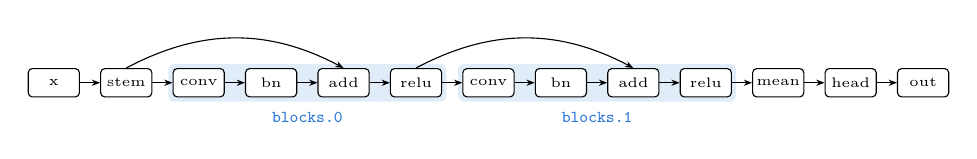
\begin{tikzpicture}[x=9.2mm]
\foreach \i/\l in {0/x,1/stem,2/conv,3/bn,4/add,5/relu,6/conv,7/bn,8/add,9/relu,10/mean,11/head,12/out}
  \node[fx] (n\i) at (\i,0) {\l};
\foreach \a/\b in {0/1,1/2,2/3,3/4,4/5,5/6,6/7,7/8,8/9,9/10,10/11,11/12} \draw[ar] (n\a) -- (n\b);
\draw[ar] (n1.north) to[bend left=28] (n4.north);
\draw[ar] (n5.north) to[bend left=28] (n8.north);
\begin{scope}[on background layer]
\node[fit=(n2)(n5), inner sep=1.5pt, fill=tagc!14, rounded corners=2pt, label={[font=\demofont, text=tagc]below:blocks.0}] {};
\node[fit=(n6)(n9), inner sep=1.5pt, fill=tagc!14, rounded corners=2pt, label={[font=\demofont, text=tagc]below:blocks.1}] {};
\end{scope}
\end{tikzpicture}\par\vspace{1pt}
{\footnotesize\textbf{(c) Hierarchical format \tg{M8}: a module tree + one small wiring graph per class}}\par\vspace{2pt}
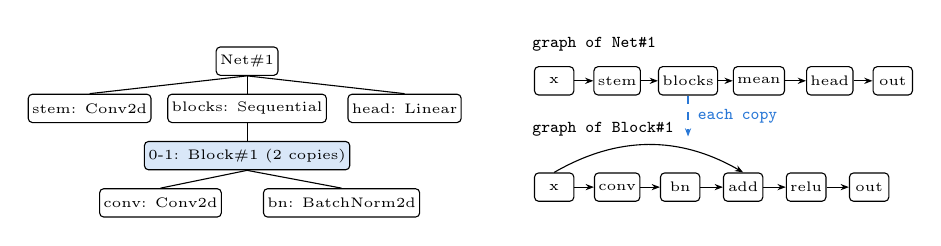
\begin{tikzpicture}[x=1mm, y=1mm, tn/.style={fx, minimum width=0pt}]
\node[tn] (net) at (19,0) {Net\#1};
\node[tn] (stem) at (-1,-6) {stem: Conv2d};
\node[tn] (blk) at (19,-6) {blocks: Sequential};
\node[tn] (head) at (39,-6) {head: Linear};
\node[tn, fill=tagc!18] (rep) at (19,-12) {0-1: Block\#1 (2 copies)};
\node[tn] (cv) at (8,-18) {conv: Conv2d};
\node[tn] (bnn) at (31,-18) {bn: BatchNorm2d};
\foreach \c in {stem,blk,head} \draw (net.south) -- (\c.north);
\draw (blk.south) -- (rep.north); \draw (rep.south) -- (cv.north); \draw (rep.south) -- (bnn.north);
\node[font=\demofont, anchor=west] at (54,2.2) {graph of Net\#1};
\foreach \i/\l/\p in {0/x/58,1/stem/66,2/blocks/75,3/mean/84,4/head/93,5/out/101}
  \node[fx, minimum width=5mm] (g\i) at (\p,-2.5) {\l};
\foreach \a/\b in {0/1,1/2,2/3,3/4,4/5} \draw[ar] (g\a) -- (g\b);
\node[font=\demofont, anchor=west] at (54,-8.6) {graph of Block\#1};
\foreach \i/\l/\p in {0/x/58,1/conv/66,2/bn/74,3/add/82,4/relu/90,5/out/98}
  \node[fx, minimum width=5mm] (h\i) at (\p,-16) {\l};
\foreach \a/\b in {0/1,1/2,2/3,3/4,4/5} \draw[ar] (h\a) -- (h\b);
\draw[ar] (h0.north) to[bend left=30] (h3.north);
\draw[ar, dashed, draw=tagc] (g2.south) -- ++(0,-5.2) node[midway, right, font=\demofont, text=tagc] {each copy};
\end{tikzpicture}
\end{minipage}
\end{minipage}
\end{document}
